Auf dem Quadrat
\begin{equation}
\Omega = \{ (x,y)\,|\, 0<x<\pi \;\text{und}\; 0 < y < \pi \}
\label{40000018:domain}
\end{equation}
soll die Differentialgleichung
\begin{equation}
\Delta u = \sin x\cos y
\label{40000018:pde}
\end{equation}
mit den Randbedingungen $u=0$ auf $\partial\Omega$ gelöst werden.
Die Lösung soll in der Form $u=u_p+u_h$ gefunden werden, wobei
$u_h$ eine Lösung der homogenen Gleichung $\Delta u_h=0$ ist.
\begin{teilaufgaben}
\item
Finden sie eine partikuläre Lösung $u_p$.
\item
Bestimmen Sie die Randbedingungen von $u_h$.
\item
Verwenden Sie einen Separationsansatz für $u_h$, stellen Sie die
Differentialgleichungen und Randbedinungen für die Faktoren auf.
\item
Lösen Sie die Differentialgleichungen.
\item
Führen Sie den Koeffizientenvergleich durch und bestimmen sie $u_h$.
\end{teilaufgaben}


\begin{loesung}
\begin{teilaufgaben}
\item
Dies ist eine inhomogene Differentialgleichung, wir brauchen also zunächst
eine partikuläre Lösung.
Die rechte Seite der Differentialgleichung ist eine Funktion, die bis auf
einen konstanten Faktor die Differentialgleichung erfüllt.
Es gilt nämlich
\[
\Delta (\sin x\cos y)
=
-\sin x\cos y - \sin ax\cos y
=
-2 \sin x\cos y
\]
Also ist
\[
u_p(x,y)
=
-\frac{1}{2} \sin x\cos y
\]
eine partikuläre Lösung der Differentialgleichung.

\item
\begin{figure}
\centering
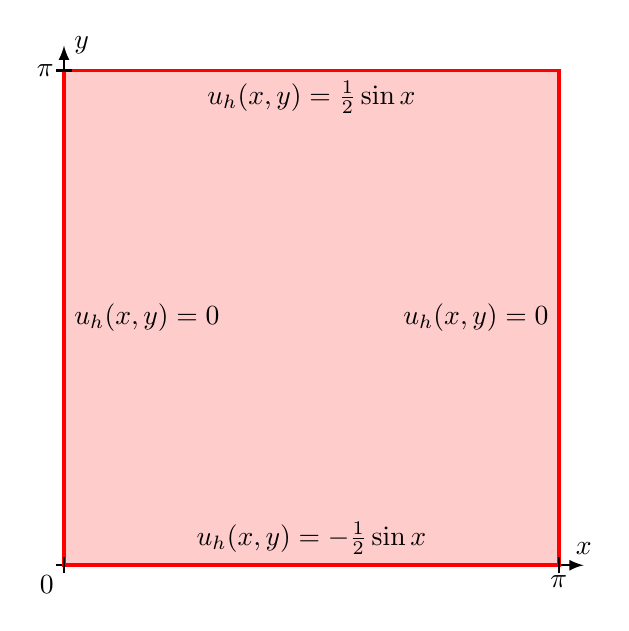
\begin{tikzpicture}[>=latex,thick]
\fill[color=red!20] (0,0) rectangle ({2*3.1415},{2*3.1415});
\draw[->] (-0.1,0)--(6.6,0) coordinate[label={$x$}];
\draw[->] (0,-0.1)--(0,6.6) coordinate[label={right:$y$}];
\draw[color=red,line width=1.4pt] (0,0)--({2*3.1415},0)--({2*3.1415},{2*3.1415})--(0,{2*3.1415})--cycle;
\draw (0,-0.1)--(0,0.1);
\draw ({2*3.1415},-0.1)--({2*3.1415},0.1);
\draw (-0.1,{2*3.1415})--(0.1,{2*3.1415});
\node at (0,{2*3.1415}) [left] {$\pi$};
\node at ({2*3.1415},0) [below] {$\pi$};
\node at (0,0) [below left] {$0$};
\node at (3.1415,0) [above] {$u_h(x,y)=-\frac12\sin x$};
\node at (3.1415,{2*3.1415}) [below] {$u_h(x,y)=\frac12\sin x$};
\node at (0,3.1415) [right] {$u_h(x,y)=0$};
\node at ({2*3.1415},3.1415) [left] {$u_h(x,y)=0$};
\end{tikzpicture}
\caption{Gebiet für die Aufgaben~\ref{40000018}
\label{40000018:gebiet}}
\end{figure}
Auf dem Rand des Gebietes $\Omega$ sind die Funktionswerte von $u_p$:
\[
u_p(0,y) = u_p(\pi,y)=0
\qquad\text{und}\qquad
u_p(x,0) = -\frac12\sin x = -u_p(x,\pi).
\]
Wir suchen daher eine Lösung der homogenen Gleichung $\Delta u_h = 0$
mit den Randbedingungen
\[
u_h(0,y) = u_h(\pi,y) = 0
\qquad\text{und}\qquad
u_h(x,0) = \frac12\sin x = -u_h(x,\pi).
\]
(Siehe auch Abbildung~\ref{40000018:gebiet}.)
\item
Zur Bestimmung der Lösung $u_h$ der homogenen Gleichung verwenden wir einen
Separationsansatz, wir setzen
\[
u(x,y) = X(x)\cdot Y(y).
\]
Diesen Ansatz setzen wir in die Differentialgleichung ein und erhalten
\[
X''(x)Y(y) + X(x)Y''(y)=0
\qquad\Rightarrow\qquad
\frac{X''(x)}{X(x)} = -\frac{Y''(y)}{Y(y)}
\]
Die Separationsmethode besagt, dass die Seiten der Gleichung konstant
sein müssen, also
\[
X''(x) = -\mu X(x)
\qquad\text{und}\qquad
Y''(y) = \mu Y(y).
\]
\item
Als Lösungen für $X$ kommen nur die Funktionen 
$\sin kx$ mit ganzzahligem $k$ in Frage.
Die Gleichung für $Y(y)$ hat die Lösungen $e^{ky}$ und $e^{ky}$.
Die allgemeine Lösung für $u_h$ ist daher
\[
u_h(x,y)
=
\sum_{k=1}^\infty \sin kx (a_k e^{ky} + b_k e^{ky})
\]
Diese Lösung erfüllt die Randbedingungen für $x=0$ und $x=\pi$.
\item
Es bleiben also noch die Randbedingungen für $y=0$ und $y=\pi$ zu erfüllen:
\begin{equation}
\begin{aligned}
u_h(x,0)   &= \sum_{k=1}^\infty \sin kx \cdot (a_k + b_k)&&=-\frac12\sin x
\\
u_h(x,\pi) &= \sum_{k=1}^\infty \sin kx \cdot (a_ke^{k\pi} + b_ke^{-k\pi}) &&=\frac12\sin x
\end{aligned}
\end{equation}
Diese Gleichungen können nur für $k=1$ erfüllt sein, dann muss gelten
\begin{equation}
\begin{linsys}{2}
       a_1&+&        b_1&=& -\frac12\\
e^{\pi}a_1&+&e^{-\pi}b_1&=&  \frac12
\end{linsys}
\end{equation}
Die Koeffizienten $a_k$ und $b_k$ kann man zum Beispiel mit der Kramerschen
Regel finden:
\begin{align*}
a_1
&=
-\frac12\cdot
\frac{e^{-\pi}+1}{e^{-\pi}-e^{\pi}}
\\
b_1
&=
\frac12\cdot
\frac{1+e^{\pi}}{e^{-\pi}-e^{\pi}}
\end{align*}
Damit haben wir für die Lösung der homogenen Gleichung
\[
u_h(x,y)
=
\frac12
\sin x \cdot \biggl(
-
\frac{e^{-\pi}+1}{e^{-\pi}-e^{\pi}} e^y
+
\frac{1+e^{\pi}}{e^{-\pi}-e^{\pi}} e^{-y}
\biggr)
\]
und für die Lösung der Differentialgleichung
\[
u_p
=
\sin x \cos y
+
\frac12
\sin x \cdot \biggl(
-
\frac{e^{-\pi}+1}{e^{-\pi}-e^{\pi}} e^y
+
\frac{1+e^{\pi}}{e^{-\pi}-e^{\pi}} e^{-y}
\biggr).
\qedhere
\]
\end{teilaufgaben}
\end{loesung}

\begin{bewertung}
\begin{teilaufgaben}
\item
Partikuläre Lösung ({\bf P}) 1 Punkt,
\item
Randbedingungen für $u_h$ ({\bf R}) 1 Punkt,
\item
Separation ({\bf S}) 1 Punkt,
\item
Lösungen für $X(x)$ und Ganzzahligkeitsbedingung ({\bf X}) 1 Punkt,
Lösungen für $Y(y)$ ({\bf Y}) 1 Punkt,
\item
Koeffizientenvergleich und Lösung ({\bf K}) 1 Punkt.
\end{teilaufgaben}
\end{bewertung}




